%%%%%%%%%%%%%%%%%%%%%%%%%%%%%%%%%%%%%%%%%%%%%%%%%%%%%%%%%%%%%%%%%%%%%%
%%%%%%%%%%%%%%%%%%%%%%%%%%%%%%%%%%%%%%%%%%%%%%%%%%%%%%%%%%%%%%%%%%%%%%
\documentclass[dvips,portrait]{seminar}             %%%%%%%%%%%%%%%%%%
                                                    %%%%%%%%%%%%%%%%%%
%%%%%%%%%%%%%%%%%%%%%%%%%%%%%%%%%%%%%%%%%%%%%%%%%%%%
% gmake afb-sig-ps
%======================
\input Energy.tex
%\def\Energy{MZ-1.8GeV (had.)}
\def\Angle{$\theta^{\bullet}$}

%%%%%%%%%%%%%%%%%%%%%%%%%%%%%%%%%%%%%%%%%%%%%%%%%%%%%%%
%%%%%%%%%%%%%%%%%%%%%%%%%%%%%%%%%%%%%%%%%%%%%%%%%%%%%%%
\begin{document}                     %%%%%%%%%%%%%%%%%%


%//////////////////////////////////////////////////////////////////////////////////
%//////////////////////////////////////////////////////////////////////////////////
%//////////////////////////////////////////////////////////////////////////////////
\begin{slide}
\titbox{{\bf\Color{Red} CEEX $\sigma$ and $A_{\rm FB}$, energy cut-off study }}

\setlength{\unitlength}{1mm}
{\small\Color{PineGreen}
  Process: $e^-e^+ \to f\bar{f}$, $f=\mu^-$, at \Energy.
  Energy cut: $v<v_{\max}$, where $v=1-M^2_{f\bar{f}}/s$.
  Scattering angle for $A_{\rm FB}$ is $\theta=$\Angle.
  No cut in \Angle. 
  E-W corr. in \KK\  according to DIZET 6.x.
  \OrderLL{\alpha^3} EEX3 matrix element in \KK\ (without ISR*FSR interf.)
  \KK{}sem is semianalytical part of \KK.
  {\tiny (Angle $\theta^{\bullet}$ is from Phys. Rev. {\bf D41}, 1425 (1990).)}
}
\begin{picture}(105,54)
\put(-2, 00){\makebox(0,0)[lb]{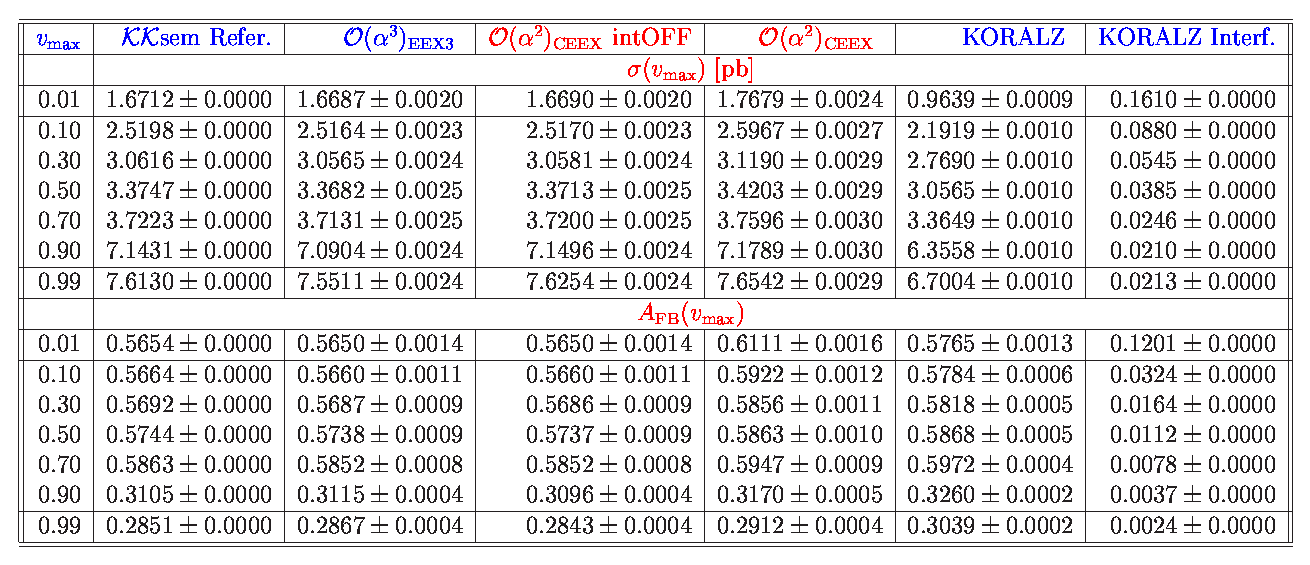
\epsfig{file=afb-int-tab1.eps,width=105mm,height=54mm}}}
\end{picture}
%-----------------------------------------------------------
\vfill
\end{slide}   %%%
%%%%%%%%%%%%%%%%%%




\end{document}

